\documentclass[11pt]{article}
\usepackage[a4paper,margin=28mm]{geometry}
\usepackage{amsmath,amssymb,amsthm,mathtools,bm}
\usepackage[T1]{fontenc}
\usepackage{lmodern,microtype}
\usepackage{graphicx,tikz,booktabs,array,longtable}
\usetikzlibrary{arrows.meta,positioning,calc}
\usepackage[numbers,sort&compress]{natbib}
\usepackage{xurl}
\usepackage[colorlinks=true,linkcolor=blue,citecolor=blue,urlcolor=blue]{hyperref}
\usepackage{bookmark,needspace}
\makeatletter
\renewcommand*\l@subsection{\@dottedtocline{2}{1.5em}{3.2em}}
\makeatother
\hypersetup{pdftitle={Random-subspace tests and trace smoothing for coordinate sweeps},pdfauthor={OpenAI}}
\newtheorem{theorem}{Theorem}[section]
\newtheorem{lemma}[theorem]{Lemma}
\newtheorem{proposition}[theorem]{Proposition}
\newtheorem{corollary}[theorem]{Corollary}
\theoremstyle{definition}
\newtheorem{definition}[theorem]{Definition}
\theoremstyle{remark}
\newtheorem{remark}[theorem]{Remark}
\DeclareMathOperator{\Tr}{Tr}
\DeclareMathOperator{\KL}{KL}
\DeclareMathOperator{\Sym}{Sym}
\DeclareMathOperator{\Var}{Var}
\DeclareMathOperator{\Ent}{Ent}
\newcommand{\TV}{\mathrm{TV}}
\newcommand{\HS}{\mathrm{HS}}
\newcommand{\op}{\mathrm{op}}
\newcommand{\E}{\mathbb E}
\newcommand{\PP}{\mathbb P}
\newcommand{\id}{\mathrm{id}}
\newcommand{\eps}{\varepsilon}
\newcommand{\ind}{\mathbf1}
\allowdisplaybreaks[1]
\setlength{\emergencystretch}{2em}
\title{Random-subspace tests and trace smoothing for coordinate sweeps}
\author{OpenAI}
\date{September 26, 2026}
\begin{document}
\maketitle
\begin{abstract}
We prove that an absolute number of coordinate sweeps of the Thorp shuffle on $n=2^d$ positions brings the full permutation to total-variation distance at most $\frac12n^{-5}$ from uniform, uniformly over the initial deck. Thus $O(d)$ physical shuffles suffice, which is optimal in order.
\end{abstract}
\tableofcontents
\section{Introduction}
A coordinate sweep sends each individual card to a uniform position, while correlations among cards remain. We study a stronger aggregate question: how small is the sum of fixed powers of all the nonconstant singular values of the full permutation operator? The answer gives a quantitative bound for repeated forward sweeps, including their multiplicities in the regular representation.

Thorp introduced the shuffle in \cite{Thorp1973}. For $n=2^d$ positions, Morris obtained an $O(d^{44})$ mixing bound using evolving sets and a chameleon process \cite{Morris2008}. Montenegro and Tetali sharpened this to $O(d^{29})$ through spectral-profile and evolving-set estimates \cite[Section~6.4]{MontenegroTetali2006}. Morris then developed an entropy method based on card interactions, obtaining $O(\log^4 n)$ for every even deck size \cite{Morris2009} and $O(d^3)$ for dyadic decks \cite{Morris2013}. These bounds count physical shuffles.

The proof here combines partial-deck smoothing with representation multiplicities and an estimate for the overlap of row and column symmetries. Splitting the binary coordinates into two consecutive groups makes one part of a sweep act independently within rows of a rectangular board and the other within columns. The two symmetry decompositions do not commute. Our geometric step estimates their overlap by testing tensor vectors against random subspaces of small dimension, and the resulting induction controls a fixed singular-value moment in the full regular representation.

\subsection{The regular-trace statement}
Index positions by $\mathbb F_2^d$. One physical shuffle sends
\[
 (x_1,x_2,\ldots,x_d)\longmapsto
 (x_2,\ldots,x_d,x_1+\xi_{x_2,\ldots,x_d}),
\]
with independent fair bits $\xi$. Removing the deterministic rotations gives a sweep through the coordinate matchings. The rotation returns to the identity after $d$ steps. Write $Q_n$ for the law of this sweep and for its average in a representation. A permutation maps inputs to outputs; a product applies its rightmost factor first. Different sweeps use independent coins.

Every matching average is an orthogonal projection, so $Q_n$ is a contraction. For $|Y|=(Y^*Y)^{1/2}$, all traces and Schatten norms are unnormalized. The regular trace on the symmetric group is
\[
 \operatorname{Tr}_{\rm reg}|Q_n|^P
 =\sum_{\lambda\vdash n}D_\lambda
       \operatorname{Tr}_{V_\lambda}|Q_n(\lambda)|^P,
\]
where $V_\lambda$ is the irreducible representation of dimension $D_\lambda$. The constant representation contributes exactly one.

\begin{theorem}[Regular-trace smoothing]\label{ten:lowplanes:main}
There is an absolute $P\ge2$ such that for every dyadic $n\ge2$,
\begin{equation}\label{ten:lowplanes:eq:1}
 \operatorname{Tr}_{\rm reg}|Q_n|^P\le1+n^{-10}.
\end{equation}
If $v$ is an integer with $2v\ge P$, then $v$ independent sweeps have total-variation distance at most $\frac12n^{-5}$ from uniform, from every deterministic initial deck. Here $\|\mu-\nu\|_{\rm TV}=\tfrac12\sum_g|\mu(g)-\nu(g)|$.
\end{theorem}
Since one sweep consists of $d$ physical shuffles, the theorem gives an $O(d)$ mixing bound for $n=2^d$ cards. This order is optimal: the support count in Proposition~\ref{ten:support} shows that total-variation distance $1/4$ requires at least $2d-O(1)$ physical shuffles.

The regular trace contains all irreducible multiplicities, not just one copy of each Fourier block. The conclusion concerns powers of the forward sweep. Its proof uses Schatten H\"older and does not identify $(Q_n^*Q_n)^v$ with $(Q_n^v)^*Q_n^v$.

\subsection{Three ranges of representations}
The proof separates three ranges, as shown in Figure~\ref{fig:three-ranges}, because the geometric test has a useful, explicit domain. If $X=\log D_\lambda$, Proposition~\ref{prop:grid-overlap} proves the overlap estimate in a window
\[
 ne^{-A_0\sqrt{\log n}}\le X\le A_1n
\]
for fixed positive $A_0,A_1$. In a balanced $a$ by $b$ board, take row and column Fourier projections selecting real unit carrier vectors, including every multiplicity copy. If their carrier dimensions are $D_R,D_F$, we prove
\[
 D_\lambda\operatorname{Tr}(E_RE_F)
 \le D_RD_F\exp\!\left(\frac{X}{(\log n)^{1/3}}\right).
\]
The test chooses independent, unitarily invariant \emph{complex} $r$-planes in the even and odd tensor alphabets, where $r=\lfloor n^{1/100}\rfloor$. The real assumption concerns the selected carrier vectors, and later permits real spectral decompositions of the sweep factors.

Two analytic estimates prepare the other ranges. Corollary~6.2 of the companion \emph{Routing densities and representation contraction for Thorp sweeps} \cite{OpenAI2026Routing} shows that a forward sweep followed by a reverse sweep, in either orientation, has a fixed power whose density on every ordered $l$-card injection is at most $e^{Cl}$. This handles very large dimensions. For diagrams with a very long first row, we break the sweep into coarse coordinate lines and deform each local operator by its polar decomposition. The two orientations of smoothing control the two ends of the singular-value decomposition. Exact uniformity for one card is preserved under this deformation. Contact counts and representation multiplicities then make the sparse regular-trace contribution at most $n^{-12}$ (Proposition~\ref{prop:sparse-rows}).

The remaining representations lie in the window of the geometric estimate. Orthogonal row and column tags turn the projection overlap into the norm of an invariant tensor. The random-plane tests retain a controlled fraction of the relevant representation. On passing both tests, nearly all slots lie in a small even subspace. Compression to the distinct cell tags then produces an exponential saving. The argument bounds arbitrary tagged vectors; it does not require them to factor across slots.

The Araki--Lieb--Thirring inequality \cite{araki1990,audenaert2007} combines the row and column estimates. An exponent increase by $1+2(\log n)^{-1/4}$ absorbs the geometric error. These increases have bounded product along the halving of bit lengths. The finite-size strict gap provides the base cases.

We use classical branching, Pieri, hook-length and ordinary Schur--Weyl theory \cite{Sagan2001,Stanley1999,VershikOkounkov2005}. The hook support of the even/odd alphabet is the classical Berele--Regev construction \cite{BereleRegev1987}, restated in \cite[Theorem~2.1]{Regev2013}. We derive the needed even/odd realization by applying ordinary Schur--Weyl separately to the two species and inducing, with a sign twist on the odd factors; the proof also tracks the exceptional letters needed outside the hook. The random-plane averaging is an application of unitary invariance and highest-weight dimension estimates. The compact coherent-orbit resolution used in the final compression is the one described by Perelomov \cite[Section~2]{Perelomov1972}; the tag construction and its quantitative trace estimate are proved here.

\begin{figure}[ht]
\centering
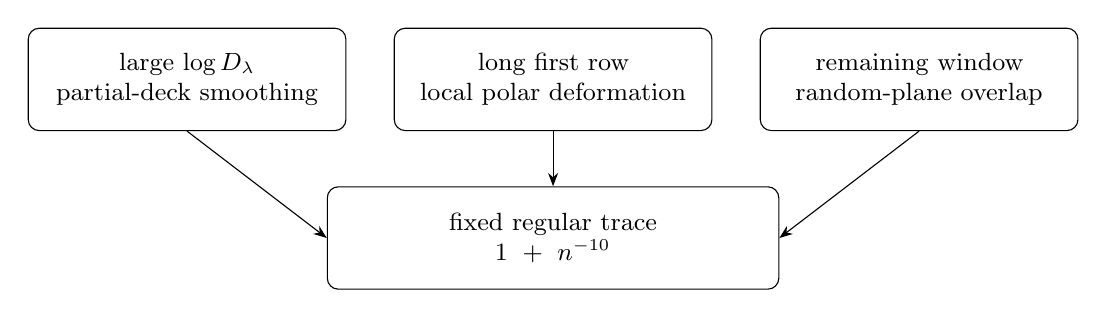
\begin{tikzpicture}[node distance=4mm,box/.style={draw,rounded corners,align=center,text width=38mm,minimum height=13mm,font=\small},>=Stealth]
\node[box] (large) {large $\log D_\lambda$\\partial-deck smoothing};
\node[box,right=6mm of large] (sparse) {long first row\\local polar deformation};
\node[box,right=6mm of sparse] (window) {remaining window\\random-plane overlap};
\node[box,below=7mm of sparse,text width=55mm] (trace) {fixed regular trace\\$1+n^{-10}$};
\draw[->] (large.south)--(trace.west);
\draw[->] (sparse.south)--(trace.north);
\draw[->] (window.south)--(trace.east);
\end{tikzpicture}
\caption{The three estimates in the proof of Theorem~\ref{ten:lowplanes:main}. After the annihilated types are removed, the cases are tested successively. The last class lies in the dimension window required by the random-plane estimate.}
\label{fig:three-ranges}
\end{figure}

\section{Coarse smoothing}
\label{ten:lowplanes:part:21}
The analytic input is the following two-orientation estimate for every partial deck. The same absolute constants apply on every coarse coordinate line used below.

\begin{proposition}[Partial-deck smoothing]\label{prop:coarse-smoothing}
Let $n=2^d$, $d\ge0$, and let $Q_n$ be a sweep in any fixed order of the distinct coordinates. For either $B_n=Q_n^*Q_n$ or $B_n=Q_nQ_n^*$, there are an absolute integer $u\ge1$ and $C<\infty$ such that
\begin{equation}
 B_n^u(x,y)\le\frac{e^{Cl}}{(n)_l},\qquad 0\le l\le n,
 \label{ten:lowplanes:eq:2}
\end{equation}
for every pair of ordered injections $x,y$ of $l$ distinct cards. Here $(n)_l=n!/(n-l)!$, including $(n)_0=1$. In particular,
\begin{equation}
 \operatorname{Tr}_{\rm reg}|Q_n|^{2u}\le e^{Cn}.
 \label{ten:lowplanes:eq:9}
\end{equation}
\end{proposition}
\begin{proof}
This is Corollary~6.2 of \citet{OpenAI2026Routing}, with its $T_N=Q_n$ and $N=n$. That result proves both products, every coordinate order, and the complete range $0\le l\le n$ with the same constants. Its proof uses the all-injection density bound of Theorem~6.1, obtained by encoding cycle closures and summing their costs over network scales. For the regular trace, take $l=n$: the injection module is the regular representation, and its $n!$ diagonal entries are each at most $e^{Cn}/n!$. Since $(Q_n^*Q_n)^u=|Q_n|^{2u}$, their sum gives the second assertion.
\end{proof}

\section{Rows close to the full size}
\label{ten:lowplanes:part:127}
Representations with a very long first row occur many times in the permutation module on a relatively small partial deck. We first bound a fixed Schatten moment on that module, then use the multiplicity to bound the contribution of these representations to the regular trace.

\begin{proposition}[Sparse-row contribution]\label{prop:sparse-rows}
There are absolute constants $M,P_s$ such that, for all sufficiently large dyadic $n$,
\begin{equation}\label{eq:sparse-contribution}
 \sum_{\substack{\lambda\vdash n\\1\le n-\lambda_1\le n e^{-M\sqrt{\log n}}}}
 D_\lambda\operatorname{Tr}_{V_\lambda}|Q_n(\lambda)|^{P_s}
 \le n^{-12}.
\end{equation}
\end{proposition}

\subsection{A deformation on partial decks}
Fix $p_0\ge4u$ with $p_0>2$, where $u$ is from Proposition~\ref{prop:coarse-smoothing}. Work on ordered placements of $q$ distinguished cards. Partition the $d$ coordinate updates into consecutive pieces of length about $\sqrt d$. There are $g=O(\sqrt{\log n})$ pieces, and the corresponding coarse coordinates have sizes $b_i\le\exp(C\sqrt{\log n})$. Updating coarse coordinate $i$ means performing a local cube sweep $Q_{b_i}$ on every line parallel to it, independently across lines.

A single line operator $Y$ preserves the identities of the cards in that line and the positions of all other cards. On a block with $l$ cards in the line, it is the $l$-card placement operator for $Q_{b_i}$. Once line memberships are fixed, parallel lines are tensor factors. These observations allow us to deform the local operators without losing the placement structure.

Write $Y=W|Y|$ and set
\[
 Y(z)=W|Y|^{p_0z/2},\qquad 0\le\Re z\le1,
\]
with the value zero on the nullspace. Let $\mathcal Q(z)$ be the product of these operators in sweep order. At $z=2/p_0$ we recover the original placement sweep. On $\Re z=0$, every factor, and hence the product, has operator norm at most one. On $\Re z=1$, singular-value Cauchy--Schwarz gives, within an $l$-card line block,
\begin{equation}
 |Y(z)_{yx}|\le
 \left((|Y|^{p_0/2})_{xx}(|Y^*|^{p_0/2})_{yy}\right)^{1/2}
 \le\frac{e^{Cl}}{(b_i)_l}.
 \label{ten:lowplanes:eq:11}
\end{equation}
The last inequality uses both orientations of Proposition~\ref{prop:coarse-smoothing}: because $p_0/2\ge2u$ and $Y$ is a contraction, the displayed positive powers are bounded by the corresponding $2u$ powers. For $l=0,1$ the exponential factor is unnecessary. A single card becomes exactly uniform after all bits in a line have been updated; its line operator is therefore the uniform projection, which the deformation leaves unchanged.

\subsection{Contact counts for the deformed kernel}
\label{ten:lowplanes:part:150}
Compare the deformed product with the kernel $K(x,y)$ obtained by using an independent uniform permutation on each coarse line. The endpoints $x,y$ determine all intermediate placements: each card takes its final value in a coarse coordinate exactly when that coordinate is updated. If an intermediate placement has a collision, both kernels vanish. Otherwise the uniform-line transition probability is the product of $1/(b_i)_l$ over the lines, with $l$ the number of distinguished cards using that line.

Let $U(x,y)$ be the sum of $l\mathbf1_{\{l\ge2\}}$ over these lines, and set it to zero for invalid paths. Thus $U$ counts card visits to lines shared with another distinguished card. The local estimate and the exact one-card bound imply, on $\Re z=1$,
\[
 |\mathcal Q(z)_{yx}|\le K(x,y)e^{CU(x,y)},
 \qquad K(x,y)\le n^{-q}e^{CU(x,y)}.
\]
For the second inequality, compare each denominator with $b_i^l$ and use
$b_i^l/(b_i)_l\le l^l/l!\le e^l$, with ratio one when $l\le1$.
Squaring the first bound and using the second for one factor of $K$ yields
\[
 \|\mathcal Q(z)\|_{\rm HS}^2
 \le\frac{(n)_q}{n^q}\,\mathbb E e^{C'U}.
\]
Here the expectation uses a uniform input placement and the independent uniform line permutations defining $K$.

To bound this expectation, condition on all line permutations and follow the paths of all $n$ inputs. Join two input paths if they use the same line in some piece. The resulting graph has maximum degree at most
\[
 \sum_i(b_i-1)\le e^{C''\sqrt{\log n}}.
\]
The distinguished paths are a uniform $q$-subset of its vertices. If $R_*$ counts selected vertices having a selected neighbor, then $U\le gR_*$.

For a degree bound $\Delta\ge1$, there are at most $n\Delta^{2(w-1)}$ connected vertex sets of size $w$: encode one by a rooted spanning-tree traversal of length $2(w-1)$. Any fixed union of $v\le q$ vertices is entirely selected with probability
\[
 \frac{(q)_v}{(n)_v}\le(q/n)^v.
\]
For $v>q$, that probability is zero.
The actual nontrivial components of the selected graph form a disjoint family of connected sets of sizes at least two. Consequently $e^{C'gR_*}$ is bounded by the sum, over all such contained families, of the products of their weights $e^{C'g w}$. Apply the preceding containment bound, then drop disjointness and bound the family sum by the exponential of the sum over single sets. For a sufficiently large absolute $C_2$, if
\[
 (q/n)e^{C_2\sqrt{\log n}}\le\tfrac12,
\]
this gives
\[
 \mathbb E e^{C'gR_*}
 \le\exp\!\left(n\sum_{w\ge2}
       \big((q/n)e^{C_2\sqrt{\log n}}\big)^w\right)
 \le\exp\!\left((q^2/n)e^{C_3\sqrt{\log n}}\right).
\]
This argument uses sampling without replacement; it does not require independent contact events.

Interpolate the operator-norm bound on $\Re z=0$ with this Hilbert--Schmidt bound on $\Re z=1$. At $z=2/p_0$ the Schatten exponent is $p_0$, so
\begin{equation}
 \operatorname{Tr}_{q\text{ placements}}|Q_n|^{p_0}
 \le\exp\!\left((q^2/n)e^{C_3\sqrt{\log n}}\right).
 \label{ten:lowplanes:eq:12}
\end{equation}
For completeness, the three-lines argument pairs $\mathcal Q(z)$ against a dual Schatten unit matrix of exponent $p_0'=p_0/(p_0-1)$. Keep its singular vectors fixed and raise its singular values to $p_0'(1-z/2)$, leaving zeros zero. The pairing matrix has trace norm one at the first boundary and Hilbert--Schmidt norm one at the second, and returns to the original dual matrix at $z=2/p_0$. Raising the interpolated norm bound to $p_0$ gives \eqref{ten:lowplanes:eq:12}.

\subsection{From placements to regular multiplicities}
\begin{proof}[Proof of Proposition~\ref{prop:sparse-rows}]
Write
\begin{equation}
 1\le k=n-\lambda_1\le ne^{-M\sqrt{\log n}},
 \qquad q=\left\lfloor k(n/k)^{1/5}\right\rfloor.
 \label{ten:lowplanes:eq:10}
\end{equation}
For $M$ sufficiently large, the hypothesis of \eqref{ten:lowplanes:eq:12} holds and its right side is at most $e^k$: indeed,
$q^2/n\le k(k/n)^{3/5}$. Also $q/k\to\infty$ and $q/n\to0$ uniformly in this range.

Put $\beta=(\lambda_2,\lambda_3,\ldots)$, a partition of $k$. The stabilizer of an ordered $q$-card placement is $S_{n-q}$, so branching identifies the multiplicity $m_\lambda$ with the number of standard tableaux of $\lambda/(n-q)$. For large $n$, the remaining first-row segment is separated from $\beta$, since $n-q\ge\beta_1$. Hence
\[
 m_\lambda=\binom qk D_\beta.
\]
The hook formula, with $\beta'$ denoting the transpose, gives
\begin{equation}
 D_\lambda=\binom nk D_\beta
 \prod_{i=1}^{\beta_1}
 \left(1+\frac{\beta'_i}{n-k-i+1}\right)^{-1}.
 \label{ten:lowplanes:eq:13}
\end{equation}
Since $\sum_i\beta'_i=k$ and $k=o(n)$, the product loses at most $k/(n-2k+1)$ in its logarithm. In particular,
\[
 \log D_\lambda\ge\tfrac12 k\log(n/k)
\]
for all sufficiently large $n$ in the range under consideration.

The multiplicity is a substantial power of the dimension. More explicitly,
\[
 \log m_\lambda\ge\tfrac15 k\log(n/k)-O(k)+\log D_\beta,
 \qquad
 \log D_\lambda\le k\log(n/k)+k+\log D_\beta.
\]
Because $\log(n/k)\to\infty$ uniformly, these inequalities imply $m_\lambda\ge D_\lambda^{1/10}$. The placement trace includes $m_\lambda$ copies of the $\lambda$ block. Combining this fact with \eqref{ten:lowplanes:eq:12}, and absorbing $e^k$ by the dimension lower bound, yields
\[
 \operatorname{Tr}_{V_\lambda}|Q_n(\lambda)|^{p_0}
 \le e^k D_\lambda^{-1/10}\le D_\lambda^{-1/20}.
\]
For any fixed large $A$, choose a fixed $P_s$ with $P_s/p_0\ge20(A+1)$. The inequality $\sum_j a_j^t\le(\sum_j a_j)^t$ for $a_j\ge0$ and $t\ge1$ then gives
\[
 D_\lambda\operatorname{Tr}_{V_\lambda}|Q_n(\lambda)|^{P_s}
 \le D_\lambda^{-A}.
\]

There are at most $2^k$ possible tails of size $k$. For $k\le\sqrt n$, the dimension lower bound makes their total contribution at most
$\sum_{k\ge1}(2n^{-A/4})^k$.
For $k>\sqrt n$, use $\log(n/k)\ge M\sqrt{\log n}$; the contribution is at most
\[
 \sum_{k>\sqrt n}
 \exp\!\left(k\log2-\tfrac12 A M k\sqrt{\log n}\right).
\]
Taking $A$ sufficiently large makes the sum of these two bounds at most $n^{-12}$ for all sufficiently large $n$, proving the proposition.
\end{proof}


\section{Angles between grid subgroup projections}
\label{ten:lowplanes:part:189}

Split the positions into an \(a\) by \(b\) grid, where \(ab=n\) and
\(\sqrt n/2\le a,b\le2\sqrt n\).  Write
\[
 R=(S_b)^a,\qquad F=(S_a)^b
\]
for the row and column subgroups.  We will bound the overlap of their
Fourier projections inside an irreducible representation \(V_\lambda\)
of \(S_n\).

Here is the precise meaning of the projections we use.  Choose a real
orthogonal irreducible representation \(V_\mu\) of \(R\), a real unit
vector \(v_R\in V_\mu\), and let \(D_R=\dim V_\mu\).  In the restriction
of \(V_\lambda\) to \(R\), let \(E_R\) act as
\[
 |v_R\rangle\langle v_R|\otimes I_{\mathcal M_\mu}
 \quad\hbox{on }V_\mu\otimes\mathcal M_\mu,
\]
and as zero on all other isotypic summands.  Thus \(E_R\) includes every
multiplicity copy \(\mathcal M_\mu\).  It is the evaluation on
\(V_\lambda\) of a fixed element of the group algebra of \(R\).
Define \(E_F\) and \(D_F\) in the same way for \(F\).

\begin{proposition}[Grid overlap]\label{prop:grid-overlap}
Fix \(A_0,A_1>0\).  For all sufficiently large \(n\), if
\begin{equation}
 ne^{-A_0\sqrt{\log n}}\le X:=\log D_\lambda\le A_1n,
 \label{ten:lowplanes:eq:14}
\end{equation}
then every pair of projections just described satisfies
\begin{equation}
 D_\lambda\operatorname{Tr}_{V_\lambda}(E_RE_F)
 \le D_RD_F\exp\!\left(\frac{X}{(\log n)^{1/3}}\right).
 \label{ten:lowplanes:eq:15}
\end{equation}
\end{proposition}

The proof turns this overlap into the \(\lambda\)-component of a unit
invariant tensor.  Orthogonal row and column tags make each slot carry
its own cell tag.  We then compare two estimates for that tensor after
random low-dimensional-subspace tests: averaging the tests retains a
controlled fraction of its \(\lambda\)-component, while the distinct
cell tags force the surviving tensor to have small norm.  By Stirling,
the conversion back to overlap costs
\begin{equation}\label{eq:grid-normalization-cost}
 \frac{n!}{|R||F|}
 \le \exp\!\bigl(n+O(\sqrt n\log n)\bigr).
\end{equation}
Compression to the cell tags will supply the compensating factor
\(\exp(-n)\).  The dimension window controls the remaining losses.
If either subgroup type is absent from the restriction of \(V_\lambda\),
the overlap is zero, so assume both occur.

\subsection{Tagged realization and overlap normalization}

Put \(r=\lfloor n^{1/100}\rfloor\).  For a partition \(\nu\), let
\(s(\nu)\) be the number of boxes below its first \(r\) rows and to the
right of its first \(r\) columns.  With \(s=s(\lambda)\), we first have
\begin{equation}
 s\le C X/\log n.
 \label{ten:lowplanes:eq:16}
\end{equation}
To see this, tile the diagram by \(r\) by \(r\) squares.  Each tile
meeting the counted boxes has a full tile one step up and to the left;
these full tiles contain at least \(s\) boxes in total.  Their standard
tableau counts multiply to a lower bound for \(D_\lambda\): order the
tiles by row and then column, and fill partial tiles in any fixed legal
way.  This respects the Young order.  The hook formula gives logarithmic
tableau count at least \(r^2(\log r-O(1))\) for each full square, proving
\eqref{ten:lowplanes:eq:16}.

We use Hilbert tensor powers of an alphabet with even and odd letter
spaces.  An adjacent transposition acts on homogeneous letters by
\[
 u\otimes v\longmapsto(-1)^{p(u)p(v)}v\otimes u,
\]
where \(p\) is parity.  This graded permutation action is unitary.
Whenever nonconsecutive slots are grouped together, we use the same
graded reordering.  In particular it carries actions within those slot
sets to tensor-product actions, and carries parity-stable tag subspaces
to the corresponding reordered tag subspaces.

An alphabet with \(r\) even and \(r\) odd good letters realizes precisely
the shapes contained in the \(r\)-hook.  With additional exceptional even
letters, a shape \(\nu\) can be realized using exactly \(s(\nu)\)
exceptional slots, provided at least \(s(\nu)\) exceptional letters are
available; it cannot be realized using fewer exceptional slots.  Here a fixed
letter content gives an induced representation with trivial factors
for even letters and sign factors for odd letters.  By Pieri, the good
even letters first supply at most \(r\) rows, and the good odd letters
add at most \(r\) vertical strips.  Each exceptional slot adds at most
one box outside the resulting hook.  Conversely, build the top \(r\)
rows by the even letters, then the remaining hook columns by the odd
letters, and finally the outside boxes with distinct exceptional letters.
This proves both assertions.

Realize \(\lambda\) with \(s\) exceptional slots and restrict to \(R\).
If the chosen \(R\)-type has row shapes \(\mu_1,\ldots,\mu_a\), it occurs
in some sector splitting these exceptional slots among the rows.
The necessary exceptional count for each row gives
\begin{equation}
 h_A:=\sum_i s(\mu_i)\le s.
 \label{ten:lowplanes:eq:17}
\end{equation}
The same argument applies to the column shapes.

For row \(i\), take a separate alphabet \(A_i\) with \(r\) good letters
of each parity and \(s(\mu_i)\) exceptional even letters, and set
\(A=\bigoplus_i A_i\).  Embed each row representation in its own
alphabet tensor power, with its required exceptional count.  The
tensor product of these embeddings realizes the whole chosen
\(R\)-representation, so it also realizes the possibly entangled vector
\(v_R\).  Denote its image by \(\psi\).  It is a unit vector with exactly
\(h_A\) exceptional slots, and the slot in row \(i\) has tag \(A_i\).
For \(g\in R\), its matrix coefficient is
\[
 f_R(g)=\langle v_R,g v_R\rangle,
\]
where \(g\) acts in the chosen row representation. Outside \(R\) the
coefficient is zero, because a permutation not preserving the rows
changes a tag.  Construct a unit column-tagged vector \(\eta\) in
\(B^{\otimes n}\), \(B=\bigoplus_j B_j\), in the same way.  Its
exceptional count is \(h_B\le s\), and its coefficient on \(F\) is
\(f_F(g)=\langle v_F,g v_F\rangle\), with \(v_F\) the real unit vector
defining \(E_F\). It is zero outside \(F\).

On \(A^{\otimes n}\otimes B^{\otimes n}\), let \(P_*\) be projection
onto diagonal invariants and let \(P_A^\lambda,P_B^\lambda\) be the
isotypic projections on the respective sides.  Put
\[
 e=\psi\otimes\eta,\qquad \phi=\sqrt{n!}\,P_*e.
\]
Only the identity contributes to the diagonal coefficient average,
since \(R\cap F=\{1\}\).  Hence \(\|\phi\|=1\).
On diagonal invariants the \(A\)-action of \(g\) equals the
\(B\)-action of \(g^{-1}\). The character formulas therefore show that
the two isotypic projections agree there.
Moreover,
\begin{equation}
 \|P_A^\lambda\phi\|^2
 =\frac{|R||F|}{D_RD_Fn!}\,
   D_\lambda\operatorname{Tr}_{V_\lambda}(E_RE_F).
 \label{ten:lowplanes:eq:18}
\end{equation}
Indeed \(P_*\) commutes with \(P_A^\lambda\), and the two averaging
formulas give the left-hand side as
\[
 \frac{D_\lambda}{n!}
 \sum_{x\in F,\ z\in R}
 \chi_\lambda(z^{-1}x)f_R(z)f_F(x).
\]
The group-algebra coefficients of \(E_R\) are
\((D_R/|R|)f_R(g)\), and similarly for \(E_F\).  The coefficients are
real and unchanged by inversion because the selected carrier vectors
are real.  Taking the trace of the product gives
\eqref{ten:lowplanes:eq:18}.

\subsection{Retention under random-plane tests}
\label{ten:lowplanes:part:243}

The good even and good odd spaces of \(A\) each have dimension \(H=ar\).
Choose an independent unitarily invariant complex \(r\)-plane in each,
and let \(V_A\) be their sum.  Let \(T_A\) project onto tensors with at
most
\[
 L_A=3s+2rH
\]
slots outside \(V_A\).  Every exceptional slot counts as outside.
Write \(\overline T_A\) for the average over the two planes.

\begin{lemma}[Retention on the isotypic sector]\label{lem:plane-retention}
On the sector with exactly \(h_A\) exceptional slots,
\begin{equation}
 \overline T_A\ge\alpha_H P_A^\lambda,
 \qquad \alpha_H=(n+H)^{-2rH}.
 \label{ten:lowplanes:eq:19}
\end{equation}
The inequality holds on all multiplicity spaces.
\end{lemma}

\begin{proof}
Fix also the counts \(k,m\) of good even and good odd slots.
Apply ordinary Schur--Weyl separately to these species.  For unitary
highest weights \(\rho\vdash k\) and \(\xi\vdash m\), the symmetric-group
side is induced from the Specht representations of \(\rho,\xi'\) and
the exceptional tensor representation: the arrangements of the three
species among the slots account for the induction.  The transpose on the odd
species is the sign twist.  If this summand contains \(\lambda\),
branching and reciprocity imply
\[
 \rho\subseteq\lambda,\qquad \xi'\subseteq\lambda.
\]
The highest weights \(\rho\) and \(\xi\) have height at most \(H\).
Both therefore have at most \(s+rH\) boxes below their first \(r\) rows.  For \(\rho\), at most \(rH\) such boxes lie in
the first \(r\) columns and the rest are counted by \(s(\lambda)\);
use \(s(\lambda')=s(\lambda)\) for \(\xi\).

For fixed planes, the two complement counts are Lie-algebra operators
on the two unitary-representation factors.  Thus the test, a spectral
projection of their sum plus \(h_AI\), acts as identity on multiplicity
spaces even before averaging.  Its average is scalar on each pair of
unitary types, with scalar equal to its relative trace for reference
planes.

For one highest weight \(\nu\), use the first \(r\) coordinate directions
as reference plane.  The highest-weight vector has complement count
\(\sum_{i>r}\nu_i\).  The \(U(H-r)\)-representation generated from it
has this same count, since the complement-count element is central for
that subgroup.  Its highest weight is
\((\nu_{r+1},\ldots,\nu_H)\).  Weyl's dimension formula gives its
dimension relative to the full representation as
\[
 \frac{\prod_{r<i<j\le H}(1+(\nu_i-\nu_j)/(j-i))}
      {\prod_{1\le i<j\le H}(1+(\nu_i-\nu_j)/(j-i))}
 \ge(n+H)^{-rH}.
\]
On the product of the two such subrepresentations, the test succeeds
because \(h_A+2(s+rH)\le L_A\).  The resulting relative trace is at
least \(\alpha_H\), proving the lemma.
\end{proof}

Use independent planes on the column side, with \(H'=br\),
\(L_B=3s+2rH'\), and the corresponding projector \(T_B\).
Diagonal averaging preserves the exceptional counts, so \(\phi\) lies
in both sectors to which the lemma applies.  The two positive operator
inequalities tensor together.  Since
\(P_A^\lambda P_B^\lambda\phi=P_A^\lambda\phi\), they yield
\begin{equation}
 \alpha_H\alpha_{H'}\|P_A^\lambda\phi\|^2
 \le \mathbb E\|(T_A\otimes T_B)\phi\|^2.
 \label{ten:lowplanes:eq:20}
\end{equation}
This is the lower bound for the tested norm.  We next obtain its upper
bound for every fixed choice of planes.

\subsection{Compression to orthogonal cell tags}
\label{ten:lowplanes:part:270}

Regroup the two alphabets into \(D^{\otimes n}\), where \(D=A\otimes B\)
has parity equal to the sum of the two parities.  The identification is
unitary and uses graded signs: moving a \(B\)-letter past a later-slot
\(A\)-letter contributes a minus sign when both are odd.  Checking
adjacent transpositions shows that the diagonal action becomes the
graded permutation action on \(D\).  The parity-preserving slot tests
are identified without additional signs.

The slot in cell \((i,j)\) now has tag
\(D_{ij}=A_i\otimes B_j\).  These \(n\) tag spaces are mutually
orthogonal, and \(e\) lies in their product tag subspace.  No
factorization of \(e\) across the slots is asserted.

Passing both tests leaves at most \(L_A+L_B\) slots outside
\(W=V_A\otimes V_B\).  The tests preserve diagonal invariants.  In an
invariant graded tensor, the number of slots in the odd part of \(W\)
is at most its dimension: after fixing their positions and grouping them,
those factors alternate.  Let \(W_0\) be the even part of \(W\), and let
\(\Delta_*\) test that at most
\[
 T=L_A+L_B+4r^2
\]
slots lie outside \(W_0\).  We obtain
\begin{equation}
 \|(T_A\otimes T_B)\phi\|^2
 \le\|\Delta_*\phi\|^2
 =n!\|P_*\Delta_*e\|^2.
 \label{ten:lowplanes:eq:21}
\end{equation}
The final equality uses the commutation of \(\Delta_*\) with the
diagonal action.  Also
\[
 \dim W_0\le4r^2,\qquad
 T\le C X/\log n<n/2
\]
for large \(n\): the terms in \(T\) not involving \(s\) are
\(O(n^{0.52})\), and the lower endpoint of
\eqref{ten:lowplanes:eq:14} absorbs them.

\begin{lemma}[Cell-tag compression]\label{lem:cell-compression}
With the notation above, put
\[
 M_*=\sum_{t\le T}\binom nt.
\]
Then
\[
 n!\|P_*\Delta_*e\|^2
 \le n!M_*^2\max_{0\le t\le T}
 \frac{\dim(\operatorname{Sym}^{n-t}W_0)}
      {t!\,(n-t)^{n-t}}.
\]
\end{lemma}

\begin{proof}
Write \(\Delta_*=\sum_{|S|\le T}\Delta_S\), where \(\Delta_S\)
specifies exactly the slots outside \(W_0\).  Fix \(S\), put
\(t=|S|\), \(m=n-t\), and group the remaining slots before those in
\(S\), using graded reordering.  Parity-stability of the tags ensures
that the reordered vector still lies in the corresponding product
tag subspace.

The full invariant projection is dominated by the product of the two
within-group invariant projections.  Since \(\Delta_S\) commutes with
these within-group projections, and we may relax the test on \(S\) to
identity, \(\|P_*\Delta_Se\|^2\) is bounded by the quadratic form of
\[
 \Pi_m\otimes\Pi_t,
 \qquad
 \Pi_m=P_{\operatorname{Sym}^m W_0},\quad
 \Pi_t=P_{\text{graded symmetric tensors in }D^{\otimes t}}.
\]
We now compress this operator to the product tag subspace.  The
compression splits into the tensor product of the two compressed
operators; no tag projection is required to commute with
\(P_{W_0}\).  On the \(S\)-slots every nonidentity permutation changes
a tag, so the compression of \(\Pi_t\) is exactly identity divided
by \(t!\).

For the other factor, unitary invariance and irreducibility give
\[
 \Pi_m=\dim(\operatorname{Sym}^mW_0)\,
 \mathbb E_z\,|z^{\otimes m}\rangle\langle z^{\otimes m}|,
\]
where \(z\) is a uniform complex unit vector in \(W_0\).  This is the
compact coherent-orbit resolution of
\citet[Section~2]{Perelomov1972}.
If \(C_\ell\) projects to the tag of remaining slot \(\ell\), then
the compressed rank-one operator has norm
\[
 \prod_{\ell=1}^m\|C_\ell z\|^2\le m^{-m},
\]
by orthogonality of the tags and arithmetic--geometric mean.
Consequently the compression of \(\Pi_m\) has norm at most
\(\dim(\operatorname{Sym}^mW_0)m^{-m}\).
The product of these two operator bounds applies to any unit vector
in the tag subspace, including the entangled vector \(e\).

Thus each assignment contributes at most the fraction in the lemma.
Cauchy--Schwarz in the sum of the \(M_*\) vectors \(P_*\Delta_Se\)
gives the additional factor \(M_*^2\), proving the result.
\end{proof}

\begin{proof}[Completion of the proof of Proposition~\ref{prop:grid-overlap}]
The number of assignments is at most
\[
 M_*\le\exp\!\bigl(C T\log(en/T)\bigr).
\]
Use \(\dim W_0\le4r^2\) and Stirling in the compression lemma.  In
particular,
\[
 \frac{n!}{t!\,(n-t)^{n-t}}
 =\binom nt\exp\!\bigl(-(n-t)+O(\log n)\bigr).
\]
We obtain
\[
 \mathbb E\|(T_A\otimes T_B)\phi\|^2
 \le
 \exp\!\left(-n+
 O\!\left(T\log(en/T)+r^2\log n\right)\right).
\]
The inverse retention factor in \eqref{ten:lowplanes:eq:20} costs
\[
 \log(\alpha_H\alpha_{H'})^{-1}=O(n^{0.6}).
\]
Finally \eqref{ten:lowplanes:eq:18} restores the subgroup normalization.
Combining these three bounds gives
\[
 \frac{D_\lambda\operatorname{Tr}(E_RE_F)}{D_RD_F}
 \le
 \exp\!\left(O\!\left(
 T\log(en/T)+r^2\log n+n^{0.6}+\sqrt n\log n
 \right)\right).
\]
Here the compression term \(-n\) cancels the \(+n\) in
\eqref{eq:grid-normalization-cost}.  The dimension window and
\(T\le CX/\log n\) imply
\[
 T\log(en/T)=O_{A_0,A_1}\!\left(\frac{X}{\sqrt{\log n}}\right);
\]
the other displayed losses are absorbed by the same bound.
For sufficiently large \(n\), this is at most
\(X/(\log n)^{1/3}\), proving \eqref{ten:lowplanes:eq:15}.
\end{proof}


\section{The uniform moment induction}
\label{ten:lowplanes:part:309}
We first remove the representations controlled by a fixed power, then show that every remaining representation lies in the window of Proposition~\ref{prop:grid-overlap}. The overlap estimate will close an induction through balanced splits of the coordinate set.

\subsection{Covering the representation ranges}
A representation of height greater than $n/2$ is annihilated by one coordinate matching. Indeed, that matching average projects onto invariants of its pair-switching subgroup. By Pieri, induction from $n/2$ trivial $S_2$ factors produces only shapes of height at most $n/2$.

For $X=\log D_\lambda\ge A_1n$, choose the absolute constant $A_1$ large enough that Proposition~\ref{prop:coarse-smoothing} gives
\[
 \operatorname{Tr}_{V_\lambda}|Q_n(\lambda)|^{2u}
 \le e^{Cn}/D_\lambda\le D_\lambda^{-1/2}.
\]
A larger fixed power makes the sum of the regular contributions in this range at most $n^{-12}$. Here we use the bound $e^{O(\sqrt n)}$ on the number of partitions of $n$, which also follows by evaluating the partition generating product at $e^{-1/\sqrt n}$. Proposition~\ref{prop:sparse-rows} supplies the same aggregate bound for long first rows. Since all singular values are at most one, we may choose a common fixed power $P_c\ge2$ for these two estimates.

Every remaining nontrivial representation satisfies
\eqref{ten:lowplanes:eq:14}, for a fixed $A_0$ chosen sufficiently large in terms of $M$. Only the lower endpoint needs proof. Suppose first that the first row or first column has length $L\ge n/8$. Transpose if necessary, preserving dimension, and retain the first row together with a subdiagram of
\[
 t=\lfloor ne^{-M\sqrt{\log n}}\rfloor
\]
boxes below it. There are enough boxes: in the row case we have excluded the sparse range of Proposition~\ref{prop:sparse-rows}; in the column case the original height is at most $n/2$, so the transposed tail has at least $n/2$ boxes. Since $t=o(L)$, the hook comparison \eqref{ten:lowplanes:eq:13}, applied to this smaller diagram, gives logarithmic dimension at least $t$ for large $n$. Branching bounds this dimension by $D_\lambda$. If both the first row and first column have length less than $n/8$, every hook is at most $n/4$, and the hook formula instead gives
\[
 D_\lambda\ge\frac{n!}{(n/4)^n},\qquad \log D_\lambda\ge cn.
\]
Both cases imply the required lower endpoint after choosing $A_0>M$.

\subsection{Closing the induction}
\begin{proof}[Proof of Theorem~\ref{ten:lowplanes:main}]
Fix a threshold $n_0$ large enough for the preceding estimates and the numerical comparisons below. For each of the finitely many dyadic sizes $2\le n<n_0$, every nonconstant regular singular value of $Q_n$ is strictly less than one. Norm equality through a product of orthogonal projections would force a common invariant vector for all coordinate switches. These switches generate $S_n$, so only constants can have equality. A common finite power, chosen at least $P_c$, therefore proves \eqref{ten:lowplanes:eq:1} for all these base sizes. Denote it by $P(n)$ there.

For a larger size $n=2^d$, split the coordinates into consecutive groups of sizes $\lfloor d/2\rfloor$ and $\lceil d/2\rceil$. They give a balanced $a$ by $b$ grid. The two sweep factors are a row law, consisting of independent $b$-card cube sweeps, and a column law, consisting of independent $a$-card cube sweeps. Set
\[
 p=\max\{P(a),P(b),P_c\},\qquad
 P(n)=\bigl(1+2(\log n)^{-1/4}\bigr)p.
\]
The already controlled classes retain their bounds at this power. Consider a remaining representation, with $X$ in \eqref{ten:lowplanes:eq:14}, and write the two factors in matrix product order as $Q_n=YZ$.

The Araki--Lieb--Thirring inequality \cite{araki1990,audenaert2007}, with exponent $p/2\ge1$, gives
\begin{equation}
 \operatorname{Tr}_{V_\lambda}|YZ|^p
 \le\operatorname{Tr}_{V_\lambda}
       (Y^*Y)^{p/2}(ZZ^*)^{p/2}.
 \label{ten:lowplanes:eq:22}
\end{equation}
The left side is the trace of the $p/2$ power of
$(Y^*Y)^{1/2}ZZ^*(Y^*Y)^{1/2}$.
Take spectral decompositions of the two positive powers on their own subgroup irreducibles and then restrict to $V_\lambda$. Real orthogonal models give real eigenvectors, so the resulting projections are exactly those covered by Proposition~\ref{prop:grid-overlap}; each projection acts on all copies of its carrier, with a nonnegative spectral coefficient.

For either subgroup, the sum of those coefficients multiplied by the carrier dimensions is its regular Schatten $p$-moment. The product subgroup laws are independent across lines, so these traces factor. Multiplying \eqref{ten:lowplanes:eq:22} by $D_\lambda$ and applying the overlap proposition and the induction hypothesis gives
\[
 D_\lambda\operatorname{Tr}_{V_\lambda}|Q_n|^p
 \le\exp\!\left(\frac{X}{(\log n)^{1/3}}\right)
       (1+b^{-10})^a(1+a^{-10})^b.
\]
The last two factors are bounded, and the lower endpoint for $X$ absorbs that constant. Thus
\[
 \operatorname{Tr}_{V_\lambda}|Q_n|^p
 \le\exp\!\left(-X+\frac{2X}{(\log n)^{1/3}}\right).
\]
Apply $\sum_j a_j^t\le(\sum_j a_j)^t$ with
$t=P(n)/p=1+2(\log n)^{-1/4}$. The increase in exponent is larger than the relative overlap loss, and for all sufficiently large $n$ we obtain
\[
 D_\lambda\operatorname{Tr}_{V_\lambda}|Q_n|^{P(n)}
 \le\exp\!\left(-\frac{cX}{(\log n)^{1/4}}\right).
\]
The lower endpoint in \eqref{ten:lowplanes:eq:14} makes this summable over all partitions, with total at most $n^{-12}$. Adding the two previously controlled classes and the trivial representation gives a total at most $1+3n^{-12}\le1+n^{-10}$, closing the induction. The comparisons used here depend on $n$ and the fixed range constants, not on the size of the base-case power; hence the initial choice of $n_0$ is legitimate.

Finally $P(n)$ is bounded uniformly. Along any branch of the recursion the bit lengths undergo floor/ceiling halving until the base range. Read in reverse, those lengths grow geometrically, so the sum of their $-1/4$ powers is uniformly bounded. The factors $1+2(\log n)^{-1/4}$ consequently have bounded product. Any fixed upper bound $P$ for $P(n)$ proves \eqref{ten:lowplanes:eq:1}.

To deduce the total-variation assertion, let $\mu_v$ be the law of $v$ independent sweeps and let $\Pi$ project onto constants in the regular representation. For an integer $v$ with $2v\ge P$, Schatten H\"older on the complement of constants gives
\[
 \|Q_n^v-\Pi\|_{\rm HS}^2
 \le\operatorname{Tr}_{\rm reg,\perp}|Q_n|^{2v}\le n^{-10}.
\]
Every row of the regular transition matrix is a translate of $\mu_v$. Therefore the precise normalization is
\[
 \|Q_n^v-\Pi\|_{\rm HS}^2
 =n!\sum_{g\in S_n}\left(\mu_v(g)-\frac1{n!}\right)^2.
\]
With $U_{S_n}$ denoting the uniform law, Cauchy--Schwarz yields
$\|\mu_v-U_{S_n}\|_{\rm TV}\le\tfrac12\|Q_n^v-\Pi\|_{\rm HS}\le\tfrac12n^{-5}$.
Relabeling gives the same bound from every deterministic initial deck.
\end{proof}

An absolute number of sweeps is $O(d)$ physical shuffles. The following support obstruction gives the matching lower order.

\begin{proposition}[Support obstruction]\label{ten:support}
After $t$ physical shuffles the total-variation distance from uniform is at least $1-2^{tn/2}/n!$. Thus mixing to distance $1/4$ requires at least $\lceil(2/n)\log_2(3n!/4)\rceil=2d-O(1)$ physical shuffles.
\end{proposition}
\begin{proof}
There are at most $2^{tn/2}$ coin strings and hence at most that many possible permutations. Test this support against uniform measure and then use Stirling's formula.
\end{proof}

\bibliographystyle{plainnat}
\bibliography{references}
\end{document}
